% ------------------------------------------------------------------------------
% LaTeX Template: Presentation Slides
% This is LaTeX template is suitable for (technical) presentations
%
% Copyright: Marius Hofert, Markus Kohm (PracTeX)
% The idea of this template came from The PracTeX Journal 2010-2
% Date: April 2011
% ------------------------------------------------------------------------------

% ------------------------------------------------------------------------------
% Modified by Zamir SUN to fit VIS of Shandong Agricultural University.
% Date: Oct 26th, 2014
% ------------------------------------------------------------------------------
% Document
% ------------------------------------------------------------------------------
\documentclass[
	paper=128mm:96mm,	% like beamer
	fontsize=11pt,					% like beamer
	pagesize,							% write page size to dvi or pdf
	parskip=half-,					% paragraphs separated half a line, no marking of line endings
	numbers=noendperiod,	% removes points for special parts (e.g. appendix)
	captions=nooneline			% do not distinguish between one or more lines in captions
	]{scrartcl}							% KOMA script (article)

% Presentation tweaks	
\linespread{1.12} 				% enlarge line space

% Color
\usepackage{xcolor}			% color package; load before tocstyle

% Page structure
\usepackage{calc}				% working with lengths, counters etc.
\usepackage[
	includeheadfoot,%
	top=3.5mm,%
	bottom=3.5mm,%
	left=5.5mm,%
	right=5.5mm,%
	headsep=6.5mm,%
	footskip=8.5mm%
	]{geometry}						% set page layout parameters
\usepackage{scrpage2}		% package for page style with not only uppercase letters in the head 
\usepackage{titlesec}			% for reducing space between ((sub)sub)sections and text
\usepackage{tocstyle}			% for adjusting table of contents
\usepackage{wallpaper}
\usepackage{graphicx}
\usepackage{CJKutf8}

% ------------------------------------------------------------------------------
% Document metadata
% Fill in your own stuff here
% ------------------------------------------------------------------------------
\newcommand*{\mytitle}{山东农业大学 \LaTeX 幻灯片模板}		% title definitino
\newcommand*{\mytitleontitlepage}{山东农业大学 \LaTeX 幻灯片模板}	% title on first page (title page)
\newcommand*{\myauthor}{Zamir SUN}				% name
\newcommand*{\mydate}{\today}						% date
\newcommand*{\myuni}{信息科学与工程学院}			% university/department

% colors
\definecolor{mygreen}{RGB}{44,85,17}				% for emphasizing text (#2c5511)
\definecolor{myblue}{RGB}{34,31,217}					% for emphasizing text (#5d90c2)
\definecolor{mybrown}{RGB}{194,164,113}			% for emphasizing text (#c2a471)
\definecolor{myred}{RGB}{255,66,56}					% for emphasizing text (#cc7b76)
\definecolor{sdaugreen}{cmyk}{0.89,0.35,0.98,0.28}
\definecolor{harvestorange}{cmyk}{0,0.45,1,0}
\newcommand*{\mygreen}[1]{\textcolor{mygreen}{#1}}
\newcommand*{\myblue}[1]{\textcolor{myblue}{#1}}
\newcommand*{\mybrown}[1]{\textcolor{mybrown}{#1}}
\newcommand*{\myred}[1]{\textcolor{myred}{#1}}
\newcommand*{\sdaugreen}[1]{\textcolor{sdaugreen}{#1}}
\newcommand*{\harvestorange}[1]{\textcolor{harvestorange}{#1}}

% ------------------------------------------------------------------------------
% Fonts
% ------------------------------------------------------------------------------
\usepackage[T1]{fontenc}	% for correct hyphenation and T1 encoding
\usepackage{lmodern}			% latin modern font

% Choose one of the following three fonts
%\usepackage{fourier}			% utopia
%\usepackage{charter}			% low-resolution roman font
\renewcommand{\familydefault}{\sfdefault}% sans serif

\usepackage[english]{babel}% for Brittish English
\usepackage{microtype}		% for character protrusion and font expansion (only with pdflatex)

% ------------------------------------------------------------------------------
% Misc
% ------------------------------------------------------------------------------ 
\usepackage{amsthm}			% theorem environments
\usepackage{bm}					% for bold math symbols
\usepackage{enumitem}		% for automatic numbering of new enumerate environments
\usepackage{graphicx}		% for including figures
\usepackage{tikz}				% sophisticated graphics package
\usepackage{tabularx}			% for special table environment (tabularx-table)
\usepackage{booktabs}		% for table layout
\usepackage[
	hypertexnames=false,		% for correct links (duplicate-error solution)
	setpagesize=false,			% to prevent change text-/paperformat for the document
	pdfborder={0 0 0},			% removes border around links
	pdfpagemode=FullScreen,% open pdf in full screen mode
   pdfstartview=Fit				% fit page to pdf viewer
]{hyperref}							% all links stay black and are thus invisible
\hypersetup{						% NOTE: If \myauthor or \mytitle contain non-us-ascii-chars you
           									% should not use them inside \hyperref.
  pdfauthor=\myauthor,%
  pdftitle=\mytitle%
}
\usepackage{lastpage}			% to denote last page in slide numbering

% ------------------------------------------------------------------------------
% Page Style
% ------------------------------------------------------------------------------

\pagestyle{scrheadings}		% activates pagestyle from scrpage2
\clearscrheadfoot					% clear head and foot of scrheadings and scrplain
\setkomafont{pageheadfoot}{\normalfont\color{black}\sffamily}% setting for page head and foot

% optical vertical centering of page contents
\makeatletter
\renewcommand*{\@textbottom}{\vskip \z@ \@plus 1fil}
\newcommand*{\@texttop}{\vskip \z@ \@plus .5fil}
\addtolength{\parskip}{\z@\@plus .25fil}% stetch parskip a lot
\makeatother

% spacings
\titlespacing{\section}{0mm}{0mm}{0mm}% space (left, before, after) between section and text
\titlespacing{\subsection}{0mm}{0mm}{-1mm}% space (left, before, after) between subsection and text
\titlespacing{\subsubsection}{0mm}{0mm}{-2mm}% space (left, before, after) between subsubsection and text
\setcounter{secnumdepth}{2}% add numbering down to subsection 

% foot
\newlength{\footheight}
\setlength{\footheight}{7mm}
\addtokomafont{pagefoot}{\footnotesize}% general setting for the foot
\setkomafont{pagenumber}{\color{black}}% setting for page foot
\ifoot{% foot left
	\hspace{-2mm}%
	\begin{tikzpicture}[remember picture,overlay]
		\node [xshift=\paperwidth/2,yshift=\footheight] at (current page.south west)[rectangle,fill,inner sep=0pt,minimum width=\paperwidth,minimum height=1.5pt,top color=sdaugreen,bottom color=sdaugreen]{};% bar 
	\end{tikzpicture}%
	\myauthor\ \raisebox{0.2mm}{$\bm{\vert}$}\ \myuni
}
\ofoot[\pagemark/\pageref{LastPage}\hspace{-2mm}]{% foot right
	\pagemark/\pageref{LastPage}\hspace{-2mm}}

% table of contents
\AtBeginDocument{\renewcaptionname{english}{\contentsname}{\large Outline}}% change name of toc
\makeatletter
\newtocstyle[noonewithdot]{nodotnopagenumber}{% define tocstyle without dots and page numbers
  \settocfeature{pagenumberbox}{\@gobble}%
}
\makeatother
\usetocstyle{nodotnopagenumber}

% theorems
\newtheoremstyle{mythmstyle}%
	{0.5em}% space above
	{0.5em}% space below
	{}% body font
	{}% indent amount
	{\sffamily\bfseries}% head font
	{}% punctuation after head
	{\newline}% space after head
	{\thmname{#1}\ \thmnote{(#3)}}% head spec
\theoremstyle{mythmstyle}
\newtheorem{theorem}{Theorem}[section]
\newtheorem{remark}[theorem]{Remark}
\newtheorem{algorithm}[theorem]{Algorithm}
\renewcommand*\proofname{Proof}
\makeatletter% correct qed adjustment

% box 
\newcommand*{\mybox}[2]{% width, content
	\par\noindent
	\begin{tikzpicture}[
		mynodestyle/.style={rectangle,draw=sdaugreen,
											 thick,inner sep=2mm,text justified,top color=white,
											 bottom color=white,above}]%
		\node[mynodestyle,at={(0.5*#1+2mm+0.4pt,0)}]{%
			\begin{minipage}[t]{#1}
				#2
			\end{minipage}%
		};
	\end{tikzpicture}%	
	\par\vspace{-1.3em}
}


% ------------------------------------------------------------------------------
% Begin document
% ------------------------------------------------------------------------------
\begin{document}
\begin{CJK*}{UTF8}{gbsn}
%
% ------------------------  SLIDE1  ----------------------------------
% Usually you do not need to change this page!
% 大多数情况下,不需要修改此页.
% --------------------------------------------------------------------
%
\thispagestyle{empty}
% background (stroke)
\CenterWallPaper{1}{ppt-main.jpg}
% content
\vbox to 2cm{}
\begin{center}
	\vspace{0.6cm}

	\color{white}\sffamily
	{\bfseries\Large\mytitleontitlepage\par}
   \vspace{0.5cm}
	\normalsize
   \myauthor\par
   \mydate\par
	\vfill
\end{center}
\clearpage
\ClearWallPaper
\ULCornerWallPaper{1}{sdau-bgbanner.jpg}
%
% SLIDE 2 ----------------------------------------------------------
%
\tableofcontents
\clearpage
%
% SLIDE 3 ----------------------------------------------------------
%
\section{说明}
本模板根据 Marius Hofert, Markus Kohm (PracTeX) 发表在\\
http://tug.org/pracjourn/2010-2/hofert.html 的模板为基础\\
结合山东农业大学视觉形象识别系统管理手册的要求,以及农大官方\\
校徽、校名题字文件为依据制作。\\
由于作者是第一次尝试使用 \LaTeX,水平有限,故难免有bug。\\
同时也因此无法提供关于 \LaTeX 的技术支持。
\clearpage
%
% SLIDE 4 ----------------------------------------------------------
%
\subsubsection*{\LaTeX 简介}
	\LaTeX is a high-quality typesetting system; it includes features designed for the production of technical and scientific documentation. \LaTeX is the \textit{de facto} standard for the communication and publication of scientific documents. \LaTeX is available as free software. (From latex-project.org)\\
\LaTeX(音译“拉泰赫”)是一种基于 \TeX{} 的排版系统,由美国计算机学家莱斯利·兰伯特(Leslie Lamport)在20世纪80年代初期开发,利用这种格式,即使使用者没有排版和程序设计的知识也可以充分发挥由 \TeX{} 所提供的强大功能,能在几天,甚至几小时内生成很多具有书籍质量的印刷品。对于生成复杂表格和数学公式,这一点表现得尤为突出。因此它非常适用于生成高印刷质量的科技和数学类文档。这个系统同样适用于生成从简单的信件到完整书籍的所有其他种类的文档。 (摘自维基百科)

\clearpage
%
% SLIDE 5 ----------------------------------------------------------
%
\section{一些例子}
\begin{enumerate}
	\item 这是一个列表示例
	\item 你可以像\sdaugreen{这样}把文字标记为\sdaugreen{山农绿 C89 M35 Y98 K28}
	\item \harvestorange{或者丰收橙 C0 M45 Y100 K0}
	\item 这两种颜色我都已经定义在了tex文件里。 
\end{enumerate}	
\clearpage
%
% SLIDE 6 ----------------------------------------------------------
%
\subsection{表格示例}
这是一个表格示例。我保留了源模板中的内容。\\
How long does it take your eye to find the largest number? How often does this number appear? Seems \myred{impossible} to decide during a talk~\dots

\begin{tabularx}{\textwidth}{@{\extracolsep{\fill}}cccccccc}
   \toprule
   \multicolumn{1}{c}{\#}&\multicolumn{1}{c}{A}&\multicolumn{1}{c}{B}&\multicolumn{1}{c}{C}&\multicolumn{1}{c}{D}&\multicolumn{1}{c}{E}&\multicolumn{1}{c}{F}&\multicolumn{1}{c}{G}\\ 
   \midrule
   1&0.7234&0.6243&0.7134&0.6143&0.7124&0.7142&0.7123\\
   2&0.7123&0.6599&0.7289&0.6904&0.7344&0.7879&0.7888\\
   3&0.7498&0.7659&0.7028&0.7728&0.7483&0.7980&0.7643\\
   4&0.7919&0.7981&0.7976&0.7433&0.7728&0.7891&0.7141\\
   5&0.7928&0.7452&0.7381&0.7948&0.7783&0.7981&0.7715\\
   \bottomrule
\end{tabularx}
\clearpage
%
% SLIDE 7 ----------------------------------------------------------
%
\subsection{图形示例}
\begin{minipage}[c]{0.8\textwidth}
\LaTeX{}可以作出非常复杂的图,这是原文的一个示例。
  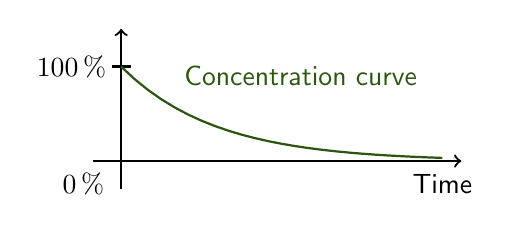
\begin{tikzpicture}[scale=1.2,thick]
    \draw[->](-3mm,0mm)--(36mm,0mm) node at (34mm,-2.4mm){Time};
    \node at (-4mm,-2.4mm){$0\,\%$};
    \draw[->](0mm,-3mm)--(0mm,14mm);
    \draw(-1mm,10mm)--(1mm,10mm) node[left=1.8mm]{$100\,\%$};
    \draw[color=mygreen,domain=0:3.4] plot(\x,{exp(-\x)});
    \node at (19mm,9mm){\mygreen{Concentration curve}};
  \end{tikzpicture}
\end{minipage}
\clearpage
%
% SLIDE 8 ----------------------------------------------------------
%
\section{编译帮助}
在Linux下可以使用pdflatex直接编译tex文件。

\clearpage
%
% SLIDE 9 ----------------------------------------------------------
%
\section{存在的问题}
\begin{enumerate}
 \item 最终生成的pdf索引中的中文乱码。
 \item 使用了CJKutf8宏包,中文字体比较少。
 \item 在Linux下使用pdflatex命令编译时,若发现页脚的总页数显示为问号,请再次编译。
\end{enumerate}
\clearpage
%
% SLIDE 10 ----------------------------------------------------------
%
\thispagestyle{empty}
% background (stroke)
\begin{tikzpicture}[remember picture,overlay]
	\node [xshift=\paperwidth/2,yshift=\paperheight/2] at (current page.south west)[rectangle,fill,inner sep=0pt,minimum width=\paperwidth,minimum height=\paperheight/3,top color=sdaugreen,bottom color=sdaugreen]{};
\end{tikzpicture}%
% content
\begin{center}
	\vspace{0.6cm}
	\color{white}\sffamily
	{\bfseries\Large
	Thanks!	
	\par}
	\vfill
%	\includegraphics[width=0.25\textwidth]{./contents/logo}%
\end{center}

% ------------------------------------------------------------------------------
% End document
% ------------------------------------------------------------------------------
\end{CJK*}
\end{document}
